\section{Scenario}\label{sec:scenario}

Most competition tests take place in the \RoboCup\AtHome\Arena, but some tests may take place outside, in a previously unknown public place.
In this section, the \Arena{} and its contents are described, including the furnishing and other information common to all tests and leagues.

\subsection{RoboCup@Home Arena}

The \RoboCup\AtHome\Arena{} is a realistic home setting (an apartment) composed of interconnected rooms.
The minimal configuration consists of:
\begin{itemize}
	\item a bedroom,
	\item a dining room,
	\item a living room, and
	\item a kitchen
\end{itemize}
There is typically one \Arena{} per league. 
Depending on the local organization, there may be multiple \Arena{}s that differ, and a robot must be prepared to perform any task in any \Arena{}.

The arena is designed to resemble a typical apartment in the hosting country, including all necessities and decorations found in a \emph{normal} home.
Note that what is considered \emph{normal} may vary by culture and location.
Decorations can include, but are not limited to, plants, mirrors, paintings, posters, plates, picture frames, wall clocks, candles with holders, and books.

\subsection{Walls, Doors, and Floor}\label{rule:scenario_walls}

The indoor home setting will be surrounded by high and low \Term{walls}{Arena walls}, which are built up using standard fair construction material.

\begin{enumerate}
	\item \textbf{Walls:} Walls are fixed and cannot be modified during the competition. The minimum wall height is \SI{60}{\centi\meter}; a maximum height is not specified, but must allow the audience to view the competition.
	\item \textbf{Doors:} Rooms are connected by doors (at least one). All doors have handles, not knobs, and can be closed at any time.
	It is expected that robots can open these doors or find alternative paths around them.
	Doors must meet minimum accessibility requirements, with a recommended width of \SI{915}{\milli\meter}.
	\item \textbf{Floor:} The floor and doorways are even, so there are no major steps or stairs. Minor variations, such as carpets, floor transitions, and small gaps (especially at doorways), can be expected.
	\item \textbf{Appearance:} The floor and walls are mostly monochromatic, but may have textures like carpets or posters on walls.
\end{enumerate}


\subsection{Furniture}\label{rule:scenario_furniture}

The \Arena{} is furnished with typical objects common to the host country.
The minimal configuration consists of:
\begin{itemize}
	\item a bed,
	\item a couch,
	\item a small table,
	\item a small dinner table with two chairs,
	\item two trash bins,
	\item an open cupboard or a small table with a television and remote control,
	\item a chest of drawers,
	\item a high cabinet with doors
	\item a bookcase, and
	\item a coat rack
\end{itemize}

The kitchen in the \Arena{} includes:
\begin{itemize}
	\item a dishwasher,
	\item a microwave,
	\item a sink, and
	\item a refrigerator (with some cans and plastic bottles inside)
\end{itemize}

A typical \Arena{} setup is shown in~\reffig{fig:scenario_arena}.
\begin{figure}[tbp]
	\centering
	\subfloat[Typical Arena]{\label{fig:scenario_arena}\includegraphics[height=46mm]{images/typical_arena.jpg}}
	\subfloat[Typical objects]{\label{fig:scenario_objects}\includegraphics[height=46mm]{images/typical_objects.jpg}}
	\caption{An example of a \RoboCup\AtHome{} scenario}\label{fig:arena}
\end{figure}

\subsubsection{Chest of drawers}

The chest of drawers has at least two drawers located between \SI{90}{\centi\meter} and \SI{120}{\centi\meter} from the floor. These drawers require U-shaped handles for easy access.

\subsubsection{High Cabinet}

A high cabinet is any shelf-like furniture where objects can be placed. The minimum distance between shelves is \SI{30}{\centi\meter}.
The Cabinet must have two side-by-side doors blocking the access to at least the lower three shelves.
These doors require U-shaped handles for easy access.

\subsubsection{Fridge}

At least one functional fridge is required in the \Arena{} and must be at least \SI{120}{\centi\meter} in size.

\subsection{Changes to the \Arena}\label{rule:scenario_changes}

Since robots should be able to function in the real world, the \Arena{} is not fixed and might change without notice.
\begin{enumerate}
	\item \textbf{Major changes:}
	Furniture that is not fully static in everyday environments may be moved slightly between tests.
	In particular, furniture will not change rooms or move drastically within a room, but a couch or table may be slightly rotated or moved. Fixed locations for such furniture items should not be assumed.
	Walls will stay in place and rooms will retain their function.
	Passages might be blocked.
	\item \textbf{Minor Changes:} Slightly moved chairs, slightly closed doors, or similar adjustments may occur at any time, even during a test.
\end{enumerate}

\def\NumObjects{30\ }
\def\NumLocations{20\ }
\def\NumNames{20\ }

\subsection{Objects}\label{rule:scenario_objects}

Some tests in the RoboCup@Home league involve recognizing and manipulating objects (see Figure~\reffig{fig:scenario_objects}).
The \TC{} will compile a list of at least \NumObjects{} objects for this purpose.
Each object will have a picture, an official name, and an \ObjectCategory{} (e.g., an \textit{Apple} is in the \textit{Fruits} category).
Most objects are lightweight and easy to grasp with one hand.
Every \ObjectCategory{} has an assigned \PredefinedLocation{}, where objects of that category are usually found during tests (for example, an \textit{Fruits} can be found on the \textit{Kitchen Table}).
These locations are announced during the \SetupDays{} (see~\refsec{chap:setup_and_preparation}).

Objects are provided at the competition for training.
Teams may keep at most five training objects at a time and for up to one hour.
Modifying the objects is not allowed.

Two types of objects are used in the tasks:
\begin{enumerate}
	\item \textbf{\KnownObjects{}:} Objects previously known to the robot, divided into:
	\begin{enumerate}
		\item \textbf{\ConsistentObjects{}:} Objects whose image appears in the list of objects.
		\item \textbf{\SimilarObjects{}:} Objects not in the list but similar enough to one of the listed objects that a person would consider them the same kind (e.g., an apple with a different color or a cloth with a different pattern).
		\item \textbf{\StandardObjects{}:} Objects chosen from the \YCBData{}.\footnote{\url{http://www.ycbbenchmarks.com/object-set/}} These are published six months in advance on the \RoboCup\AtHome{} website\footnote{\url{https://athome.robocup.org/standard-objects}}, for teams to acquire and train on beforehand.
	\end{enumerate}
	\item \textbf{\UnknownObjects{}:} Any other object not in the object list but can be grasped or handled (e.g., \Arena{} decorations).
\end{enumerate}

The minimal configuration of \KnownObjects{} consists of:
\begin{itemize}
	\item \textbf{\iterm{Tableware}:} Dish, bowl, cup (or mug), and napkin (see Figure~\ref{fig:scenario_container_bowl}).
	\item \textbf{\iterm{Cutlery}:} Fork, knife, and spoon.
	\item \textbf{\iterm{Trash Bags}:} Large plastic trash bags, preferably with a handle.
	\item \textbf{\iterm{Bags}:} Lightweight and with stiff, vertical handles (see Figure~\ref{fig:scenario_container_bag}).
	\item \textbf{\iterm{Dry Food Container}:} Dry food containers (see Figure~\ref{fig:scenario_container_dry}).
	\item \textbf{\iterm{Disks or books}:} A set of discs (LP, CD, DVD, or BluRay) or books.
	\item \textbf{\iterm{Coat rack}:} A rack or pole to hang coats and other clothes.
	\item \textbf{\iterm{Trays}:} A transport objects like trays or baskets, intended for bimanual manipulation (see Figure~\ref{fig:scenario_container_tray}).
	\item \textbf{\iterm{Pourable}:} An object whose content can be poured (such as a cereal box).
	\item \textbf{\iterm{Heavy object}:} Weighing between \SI{1.0}{\kg} and \SI{1.5}{\kg}.
	\item \textbf{\iterm{Tiny object}:} A lightweight object not larger than \SI{5}{\centi\meter} (such as paper, a teabag, or a pen).
	\item \textbf{\iterm{Fragile object}:} An object that is easy to break (such as a chocolate egg).
	\item \textbf{\iterm{Deformable object}:} A flexible object that may change shapes (such as cloth).
	\item \textbf{\iterm{Garbage bag}:} A garbage bag that can be tied.
\end{itemize}

\begin{figure}[H]
	\centering
	\subfloat[Cereal bowls]{
		\includegraphics[width=0.24\textwidth]{images/container_bowl.png}\label{fig:scenario_container_bowl}}
	\subfloat[Bright-colored paper bags]{
		\includegraphics[width=0.24\textwidth]{images/container_paper_bag.png}\label{fig:scenario_container_bag}}
	\subfloat[Serving tray]{
		\includegraphics[width=0.24\textwidth]{images/container_tray.png}\label{fig:scenario_container_tray}}
	\subfloat[Dry food Container]{
		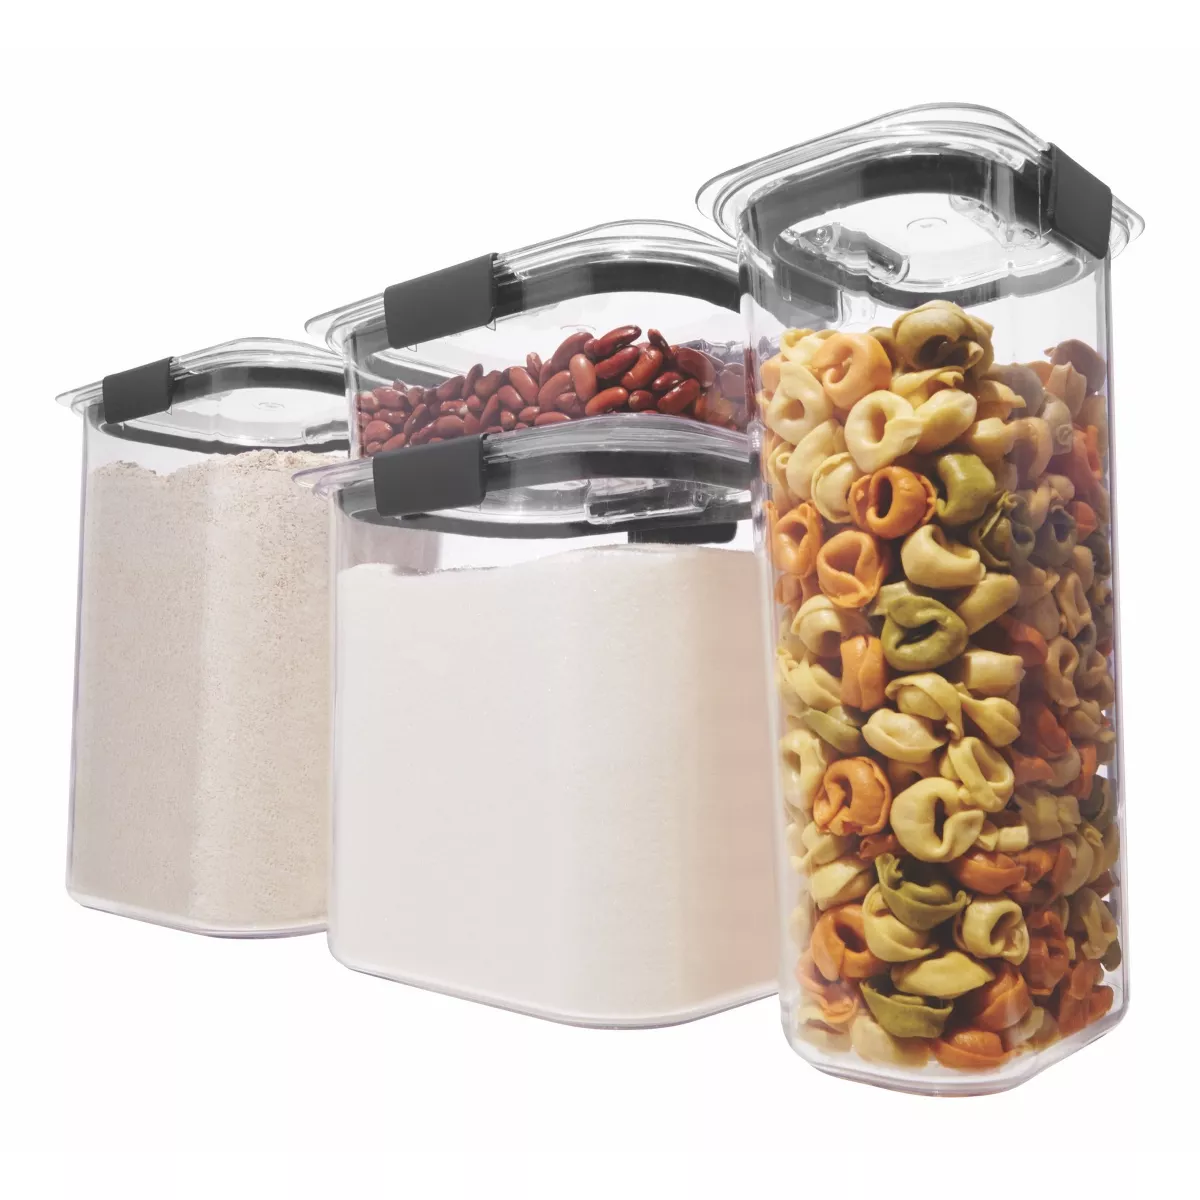
\includegraphics[width=0.24\textwidth]{images/container_dry.png}\label{fig:scenario_container_dry}}
	\caption{Example of object containers}
	\label{fig:scenario_containers}
\end{figure}

During the competition, objects can be requested based on their \ObjectCategory{}, physical attributes, or a combination of both.
Relevant attributes to be used are:
\begin{itemize}
	\item Color (such as red, blue, black with white dots, etc.).
	\item Relative estimated size (smallest, largest, big one, etc.).
	\item Relative estimated weight (lightest, heaviest).
	\item Relative position to other objects (left of, rightmost, etc.).
	\item Description (is fragile, is a container, can be poured, requires two hands, etc.).
\end{itemize}

\noindent\textbf{Remark:} Measurements are estimations and based on common sense. It is acceptable for robots to consider similar objects to be about the same size or weight.

%%%%%%%%%%%%%%%%%%%%%%%%%%%%%%%%%%%%%%%%%%%%%%%%%%%%%%%%%%%%%%%%%%
%
% Predefined locations section.
%
%%%%%%%%%%%%%%%%%%%%%%%%%%%%%%%%%%%%%%%%%%%%%%%%%%%%%%%%%%%%%%%%%%

\subsection{Predefined Rooms and Locations}\label{rule:scenario_locations}

Some tests require robots to interact with \PredefinedLocation{} where people or objects may be found.
The \Arena{} includes at least two \Term{doors}{Arena doors}, named \Entrance{} and \Exit{}, which connect to and from the \Arena{}.

Room names, predefined locations, and location classes are announced during the \SetupDays{} (see~\refsec{chap:setup_and_preparation}).

\subsection{Predefined Person Names}\label{rule:scenario_names}

Some tests involve memorizing a person's name.
Each person in the \Arena{} is assigned a \PredefinedName{} by the \TC{}.
The list of names contains \SI{25}{\percent} male, \SI{25}{\percent} female, and \SI{50}{\percent} gender-neutral names taken from the list of most commonly used names in the United States.
Predefined names are announced during the \SetupDays{} (see~\refsec{chap:setup_and_preparation}).

\subsection{Wireless network}\label{rule:scenario_wifi}

For wireless communication, an \ArenaNetwork{} is provided.
The actual infrastructure depends on the local organization.
Reliability and performance of the network are not guaranteed, so robots are expected to be able to function without it.

The following rules apply:
\begin{itemize}
	\item Only the \ArenaNetwork{} can be used during tests.
	\item Only the active team in a task is allowed can use the \ArenaNetwork{}.
	\item The \ArenaNetwork{} provides one Virtual Local Area Network (VLAN) per team.
	\item Each VLAN has its own SSID and password.
	\item VLAN traffic is isolated from others teams.
	\item Each VLAN is also connected to the Internet.
\end{itemize}

Teams broadcasting unauthorized wireless networks will be disqualified.
This includes networks with concealed SSIDs.
It is recommended to check all devices for any unauthorized wireless network activity.


